\section{Metodología de trabajo e implementación}
En esta sección en primer lugar hablamos sobre la metodología de trabajo que utilizamos durante todo el proyecto. En segundo lugar describimos las tecnologías utilizadas para el desarrollo de cada una de las partes de la aplicación: el \textit{front-end} (interfaz de usuario), el \textit{back-end} (lógica del negocio e interacción con la base de datos) y la base de datos. Finalmente describimos las arquitecturas que utilizamos.

\subsection{Metodología de trabajo}
Decidimos darle al desarrollo un enfoque ágil\cite{Shore}. Así dar visibilidad constante a todos los interesados fue uno de los principios transversales a todo el proyecto. La comunicación fue muy fluida, tanto por email, como a través de reuniones presenciales o virtuales (en forma remota). Otro de los pilares del enfoque ágil fue trabajar en forma iterativa e incremental. Es decir que trabajamos con iteraciones de tiempo fijo de una semana de duración. Al final de cada iteración los avances eran validados por el Dr. Reggiani.

\subsubsection{Resumen del itinerario del proyecto}\label{cap:itinerario}
Lo primero que hicimos fue varias reuniones entre todos los interesados en el proyecto: los desarrolladores, los directores y el Dr. Reggiani. De esas reuniones y de una visita al hospital obtuvimos los requerimientos los cuales plasmamos en forma de historias de usuario\footnote{Una historia de usuario es una representación de un requisito de software escrito en una o dos frases utilizando el lenguaje común del usuario. Las historias de usuario son utilizadas en las metodologías de desarrollo ágiles para la especificación de requisitos (acompañadas de las discusiones con los usuarios y las pruebas de validación). Hay varios formatos de historias de usuario, el que nosotros utilizamos es el siguiente: ``Como  $<$un rol$>$ quiero $<$un objetivo$>$''. Por ejemplo: ``Como enfermero quiero poder ingresar los síntomas que presenta el paciente''}.

El segundo paso fue la elección de las tecnologías (detallamos la misma más adelante en la sección \ref{cap:eleccion_tecnologias}).

En tercer lugar hicimos una estimación relativa a grandes rasgos donde calculamos cuánto tiempo iba a demandar cada funcionalidad requerida y la fecha de cierre del proyecto. Luego hicimos una planificación en donde ordenamos los requerimientos dentro de las iteraciones según las prioridades del Dr. Reggiani (ver figura \ref{fig:planificacion}).

\begin{figure}
  \centerline{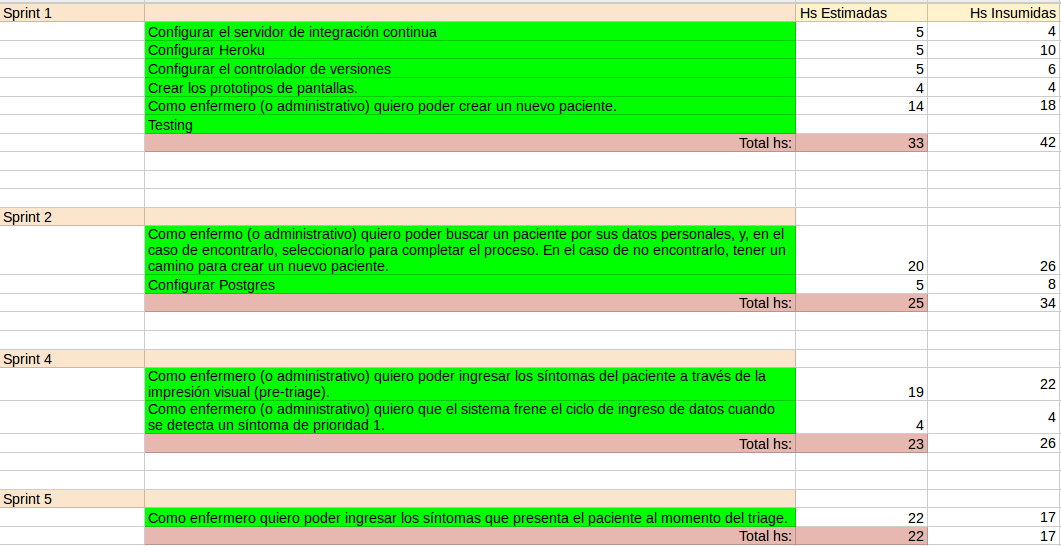
\includegraphics[width=1.2\textwidth]{planificacion.png}}
  \caption{Planificación}
  \label{fig:planificacion}
\end{figure}

A partir de ahí comenzamos con el desarrollo recorriendo las iteraciones planificadas. Al promediar el proyecto hicimos una instalación de prueba en el hospital, y al finalizar el mismo hicimos la instalación definitiva del producto terminado en una máquina de dicha institución.

\subsubsection{Flujo de trabajo en una iteración}
Al inicio de cada iteración estimamos cuanto tiempo nos llevaría cada tarea y enviamos un email con los detalles sobre lo que haríamos durante esa semana. Hacíamos prototipos de las pantallas a realizar que eran validados por el Dr. Reggiani. Dejamos sentado en una hoja de cálculo los detalles de cada tarea: el tiempo de realización estimado, la fecha de realización y el tiempo real insumido (ver figura \ref{fig:tracking}). Luego de cada avance enviamos un reporte por email informando lo realizado y si habían surgido contratiempos. Al finalizar la iteración, enviamos otro email con los detalles de las tareas finalizadas, las que estaban en progreso y las que habían quedado pendientes.

\begin{figure}[h]
  \centerline{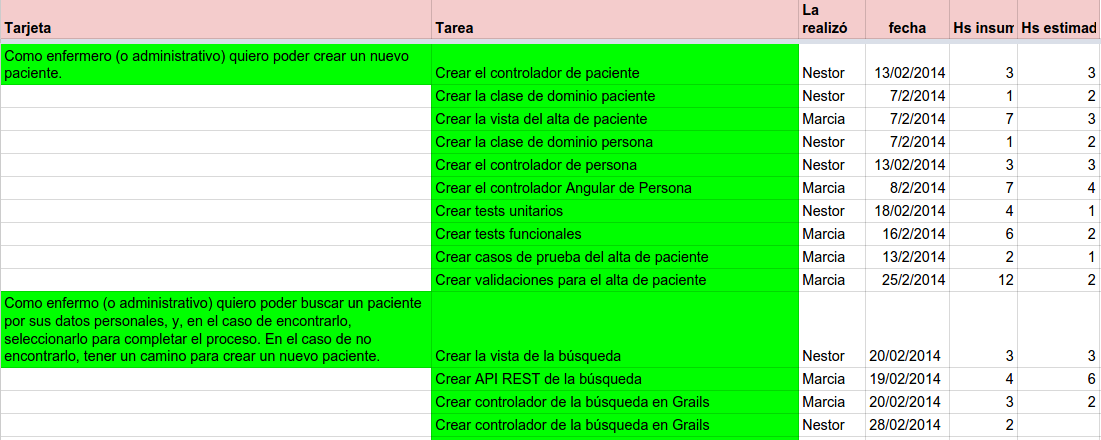
\includegraphics[width=1.2\textwidth]{tracking.png}}
  \caption{\textit{Tracking} de tareas}
  \label{fig:tracking}
\end{figure}

\subsubsection{Herramientas que utilizamos}
Detallamos a continuación las herramientas que utilizamos durante el trabajo.
\begin{itemize}
\item Google Groups\footnote{https://groups.google.com}: comunicación vía email.
\item Google Drive\footnote{https://drive.google.com/}: compartir documentación en línea.
\item Skype\footnote{http://www.skype.com.ar/es/} y Google Hangouts\footnote{https://plus.google.com/hangouts}: comunicación oral de forma remota.
\item Balsamiq\footnote{https://balsamiq.com/}: hacer prototipos de pantallas.
\item Git\footnote{http://git-scm.com/} y Github\footnote{https://github.com/}: versionar y compartir el código.
\item Travis\footnote{https://travis-ci.org/}: servidor de integración continua\footnote{http://es.wikipedia.org/wiki/Integración\_continua}.
\end{itemize}

\subsection{Tecnologías}
Todas las tecnologías que utilizamos en el desarrollo de la aplicación son de código abierto. Para desarrollar el \textit{front-end} elegimos AngularJS\footnote{https://angularjs.org/} y para el \textit{back-end} elegimos Grails\footnote{https://grails.org/}.

Cabe aclarar que ambos frameworks cubrieron ampliamente todo lo que nosotros necesitábamos de ellos para hacer este trabajo, por ello sólo utilizamos una pequeña parte de los mismos. Por ejemplo, de Grails casi no utilizamos la parte de las vistas ya que las mismas las desarrollamos del lado del cliente en AngularJS.

Además de estas dos tecnologías utilizamos Bootstrap\footnote{http://getbootstrap.com/} para obtener un diseño amigable para el usuario. Este framework también nos permitió realizar una aplicación \textit{responsive}\footnote{El diseño web adaptable o adaptativo, conocido por las siglas RWD (del inglés, Responsive Web Design) es una filosofía de diseño y desarrollo cuyo objetivo es adaptar la apariencia de las páginas web al dispositivo que se esté utilizando para visualizarla (http://es.wikipedia.org/wiki/Diseño\_web\_adaptable)} que se adapta a cualquier tamaño de pantalla, incluso de teléfonos celulares.

\subsubsection{Sobre la elección de las tecnologías}\label{cap:eleccion_tecnologias}
Como mencionamos anteriormemnte en la sección \ref{cap:itinerario} una de las primeras tareas que realizamos en el proyecto fue la elección de las tecnologías a utilizar. Entre el vasto abanico de posibilidades NodeJS\footnote{http://nodejs.org/} y Grails aparecían como las predilectas ya que son tecnologías modernas y teníamos buenas referencias de ambas. Para decidirnos por una de las dos, desarrollamos un conversor web muy simple de Farenheit a Celcius y en base a los resultados optamos por usar Grails ya que se asemeja más que NodeJS a las tecnologías que veníamos utilizando en las distintas materias a lo largo de la carrera.

Si bien Grails es \textit{full stack}\footnote{Se dice que una tecnología es \textit{full stack} cuando posee todas las herramientas necesarias para desarrollar una aplicación.}, decidimos utilizar una tecnología que resuelva las vistas del lado del cliente, se comunique con el \textit{back-end} mediante una interfaz REST\footnote{La Transferencia de Estado Representacional (Representational State Transfer) o REST es una técnica de arquitectura software para sistemas hipermedia distribuidos como la World Wide Web (http://es.wikipedia.org/wiki/Representational\_State\_Transfer)} 
y sea \textit{responsive}. Así surgió la idea de utilizar AngularJS que cubre ampliamente todos esos requisitos.

Para la elección de la base de datos nos basamos en un tutorial en línea\footnote{https://devcenter.heroku.com/articles/getting-started-with-grails} que recomienda PostgreSQL\footnote{http://www.postgresql.org.es/} como la mejor opción para usar junto a Grails.

\subsubsection{Sobre el \textit{front-end}}
El framework de aplicaciones web AngularJS es desarrollado y mantenido por Google. Es de código abierto y está escrito en JavaScript. La primer versión fue lanzada en el año 2010 y desde ese momento viene ganando espacio en la industria. Este framework es un conjunto de herramientas para la creación de aplicaciones web de una sola página (\textit{single-page applications}). Maneja contenido dinámico y permite extender el vocabulario HTML\footnote{http://es.wikipedia.org/wiki/HTML} obteniendo un entorno más expresivo, legible y práctico para el programador. La filosofía de AngularJS es que la programación declarativa es la que debe utilizarse para generar interfaces de usuario.

\subsubsection{Sobre el \textit{back-end}}
El framework de aplicaciones web Grails es \textit{full stack}, de código abierto y está hecho para la máquina virtual de Java (JVM). Está escrito en Groovy, un lenguaje de programación que a su vez está desarrollado en Java. Uno de sus principios es la convención sobre la configuración que busca decrementar el número de decisiones que un desarrollador necesita tomar, ganando así en simplicidad pero no perdiendo flexibilidad por ello. La primer versión fue lanzada en el año 2006.

Como está desarrollado en Java, Grails es multiplataforma. Además toma de su lenguaje padre tecnologías ampliamente utilizadas en la industria como Hibernate\footnote{http://es.wikipedia.org/wiki/Hibernate}, para la persistencia de datos, y Spring\footnote{http://es.wikipedia.org/wiki/Spring\_Framework}, para la seguridad, la autenticación, las pruebas, la gestión de transacciones, etc.

\subsubsection{Sobre la base de datos}
Para desarrollar una aplicación como la requerida se hizo indispensable utilizar una base de datos para almacenar toda la información ingresada. Los pacientes, los síntomas, las prioridades, los tiempos de espera, etc. son almacenados en una base de datos.

Durante todo el desarrollo de la aplicación utilizamos una base de datos H2\footnote{http://www.h2database.com} que viene embebida en Grails especialmente para utilizar en la etapa de desarrollo. También utilizamos esa tecnología en la instalación de prueba en el hospital. Pero para la instalación definitiva no utilizamos H2 ya que consideramos más apropiado y seguro tener una base de datos independiente del resto del sistema. Por eso utilizamos PostgreSQL\footnote{http://www.postgresql.org.es/} que es un sistema de gestión de bases de datos relacional orientado a objetos.


\subsection{Arquitectura}
Debido a que teníamos que desarrollar una aplicación web capaz de accederse concurrentemente desde varias máquinas al mismo tiempo, decidimos usar una arquitectura cliente-servidor\footnote{http://es.wikipedia.org/wiki/Cliente-servidor} con AngularJS del lado del cliente y Grails del lado del servidor. La comunicación se da mediante peticiones HTTP\footnote{http://es.wikipedia.org/wiki/Hypertext\_Transfer\_Protocol} desde el cliente al servidor y la información viaja en formato JSON\footnote{http://es.wikipedia.org/wiki/JSON}.


\subsubsection{Arquitectura del \textit{front-end}}
El framework AngularJS sigue el patrón de arquitectura Modelo-Vista-Controlador (MVC) de ingeniería de software y alienta la articulación flexible entre la presentación, los datos y los componentes lógicos. Con el uso de la inyección de dependencias, AngularJS lleva servicios tradicionales del lado del servidor, tales como controladores dependientes de la vista, a las aplicaciones web del lado del cliente. En consecuencia, gran parte de la carga en el \textit{backend} se reduce, lo que lleva a aplicaciones web mucho más ligeras.

\subsubsection{Arquitectura del \textit{back-end}}
El framework Grails, al igual que AngularJS, también sigue el patrón de arquitectura MVC. En lo que se refiere a la vista, como en este caso desarrollamos una aplicación de una sola página, entonces tenemos una única pantalla. Por el lado de los controladores tenemos uno por cada clase de dominio. La función principal de los controladores es procesar y responder las peticiones HTTP que llegan desde el lado del cliente. Para hacer esto el controlador se apoya en su clase de dominio (ver figura \ref{fig:diagrama_de_clases}) correspondiente y ésta, a su vez, es la que se encarga de interactuar con la base de datos.

\begin{figure}
\centerline{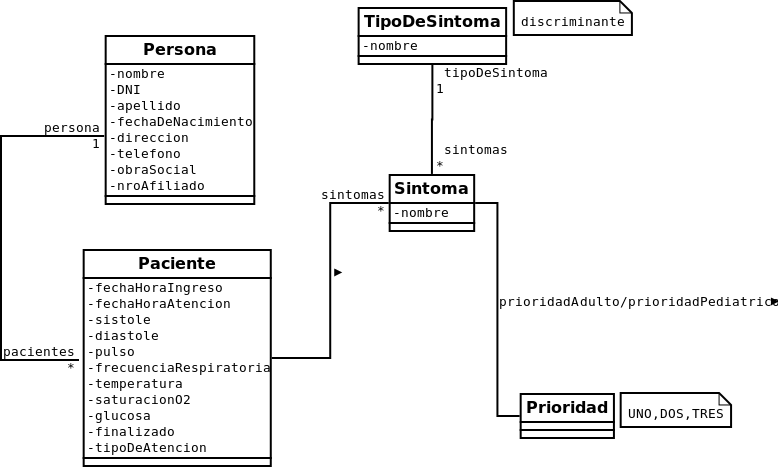
\includegraphics[width=1.2\textwidth]{triage.png}}
\caption{Diagrama de clases del dominio}
\label{fig:diagrama_de_clases}
\end{figure}